% !TEX root = ../report.tex

\appendix
\clearpage

\chapter{Data}\label{app:req}
    \begin{table}[H]
        \centering
        \begin{tabular}{l|l}
            \toprule
            \emph{Variable}        & \emph{Example}   \\
            \midrule
            \emph{app\_version}   &   0.3  \\
            \emph{user\_agent}"   &   "SOBAZAR 0.3 (iPhone; iPhone OS 6.1.4; Scale/2.00; nb\_NO)"   \\
            \emph{product\_type}  &   "product"    \\
            \emph{server\_time\_stamp} &   "2013-10-24T11:33:17.632Z"   \\
            \emph{dy}    &   24   \\
            \emph{origin\_ui} &   "storefront"     \\
            \emph{currency}  &   "kr"     \\
            \emph{country\_name}  &   "Norway"     \\
            \emph{price} &   1995     \\
            \emph{product\_name}  &   "DWS No47"   \\
            \emph{tag\_name}  &   "NULL"   \\
            \emph{tag\_id}    &   "NULL"   \\
            \emph{storefront\_name}   &   "BIK BOK"    \\
            \emph{event\_id}  &   "product\_purchase\_intended"  \\
            \emph{age\_target}    &   "Any"    \\
            \emph{epoch\_day} &   16002    \\
            \emph{mo}    &   10   \\
            \emph{yr}    &   2013     \\
            \emph{product\_id}    &   2298002  \\
            \emph{event\_location}    &   Geo Location     \\
            \emph{ipAddress} &   IP  \\
            \emph{contentDescription}    &   null     \\
            \emph{sessionId} &   null     \\
            \emph{contentId} &   null     \\
            \emph{instKey}   &   "ed4c76251ac47da54299d8c0bce3dca6"   \\
            \emph{viewer}    &   null     \\
            \emph{ts}    &   NumberLong("1382614397632")  \\
            \emph{gender\_target} &   "Female"     \\
            \emph{client\_time\_stamp} &   "NULL"   \\
            \emph{login\_type}    &   "NULL"   \\
            \emph{transaction\_id}    &   "N/A"    \\
            \emph{service\_id}    &   "SOBAZAR"    \\
            \emph{platform}  &   "iPhone"     \\
            \emph{epoch\_week}    &   2286     \\
            \emph{storefront\_id} &   23002    \\
            \emph{hr}    &   11   \\
            \emph{tag\_position}  &   "NULL"   \\
            \emph{time\_stamp}    &   "2013-10-24T13:33+0200"  \\
            \emph{retailer\_brand}    &   13001    \\
            \emph{storefront\_position}   &   2    \\
            \emph{user\_id}   &   1342189870   \\
            \emph{country\_id}    &   194001   \\
            \emph{server\_environment}    &   "prod" \\
            \bottomrule
        \caption[Complete List of Event Metadata]{Table of the complete list of event metadata stored when an event is triggered}
        \label{table:completeEventData}
        \end{tabular}
    \end{table}

    \begin{table}[H]
        \centering
        \begin{tabular}{l}
            \toprule
            \emph{Event Name}   \\
            \midrule
            \emph{activity\_clicked}  \\
            \emph{storefront\_clicked}  \\
            \emph{product\_detail\_clicked}  \\
            \emph{user\_logged\_in}  \\
            \emph{featured\_collection\_clicked}  \\
            \emph{app\_started}  \\
            \emph{featured\_storefront\_clicked}  \\
            \emph{product\_wanted}  \\
            \emph{around\_me\_clicked}  \\
            \emph{menu\_opened}  \\
            \emph{end:app\_backgrounded}  \\
            \emph{app\_became\_active}  \\
            \emph{wantlist\_menu\_entry\_clicked}  \\
            \emph{content:interact:item\_scroll}  \\
            \emph{navigation:paging\_triggered}  \\
            \emph{content:explore:user\_logo\_clicked}  \\
            \emph{collection\_viewed}  \\
            \emph{stores\_map\_clicked}  \\
            \emph{product\_purchase\_intended}  \\
            \emph{friend\_invited}  \\
            \emph{store\_clicked}  \\
            \emph{facebook\_login\_failed}  \\
            \emph{end:app\_closed}  \\
            \emph{content:explore:search}  \\
            \emph{navigation:navbar:sobazaar\_icon}  \\
            \emph{app\_first\_started}  \\
            \bottomrule
        \caption[List of Different Events]{Table of the different events that can be triggered by the user and an explanation}
        \label{table:events}
        \end{tabular}
    \end{table}


    \begin{figure}[H]
        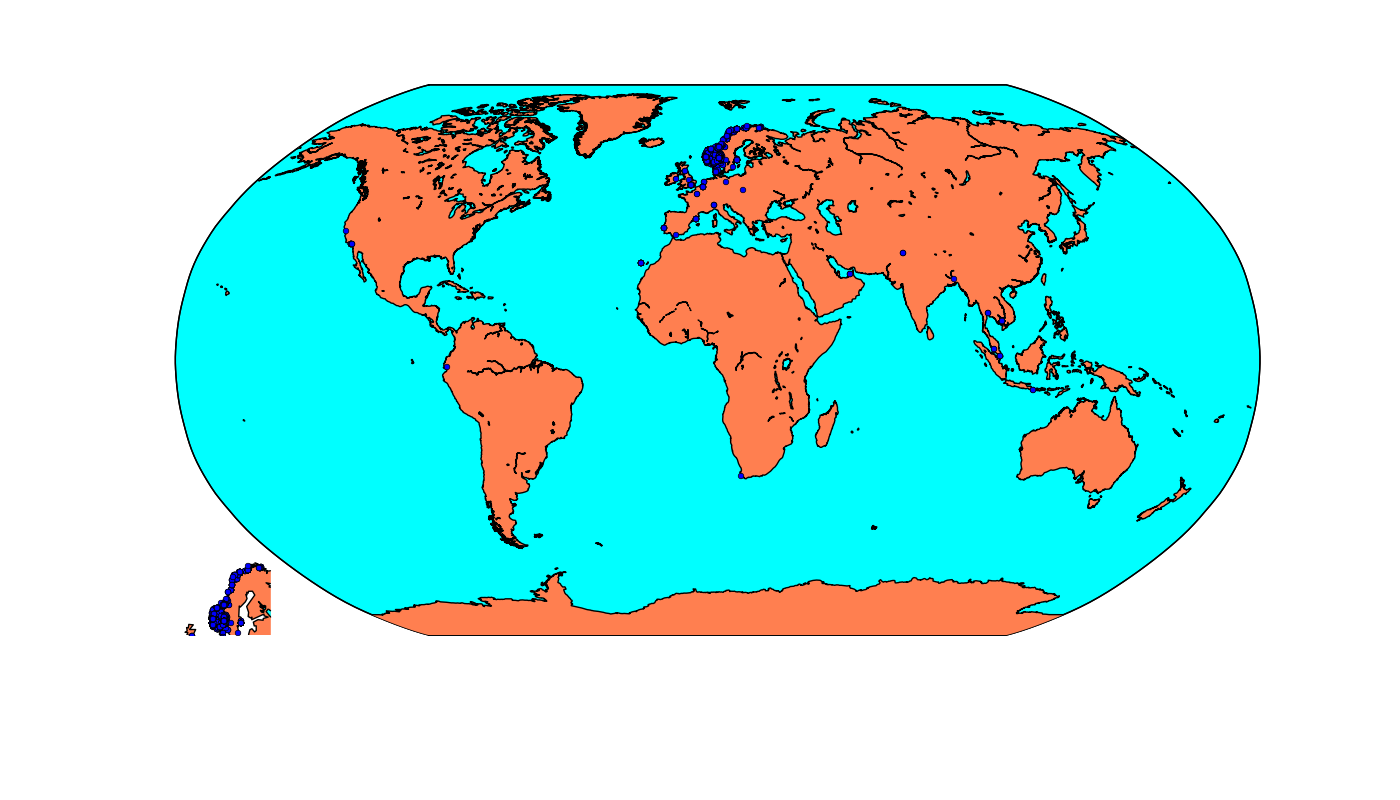
\includegraphics[width=5in]{image/simpleGeoPlotworld.png}
        \centering
        \caption[Event location mapped on the world]{This figure shows the location of the events from all over the world.
        For a cropped version with focus on Norway and the surrounding countries, refer to~\ref{figure:croppedGeoplot}}
    \end{figure}

    \begin{figure}[H]
        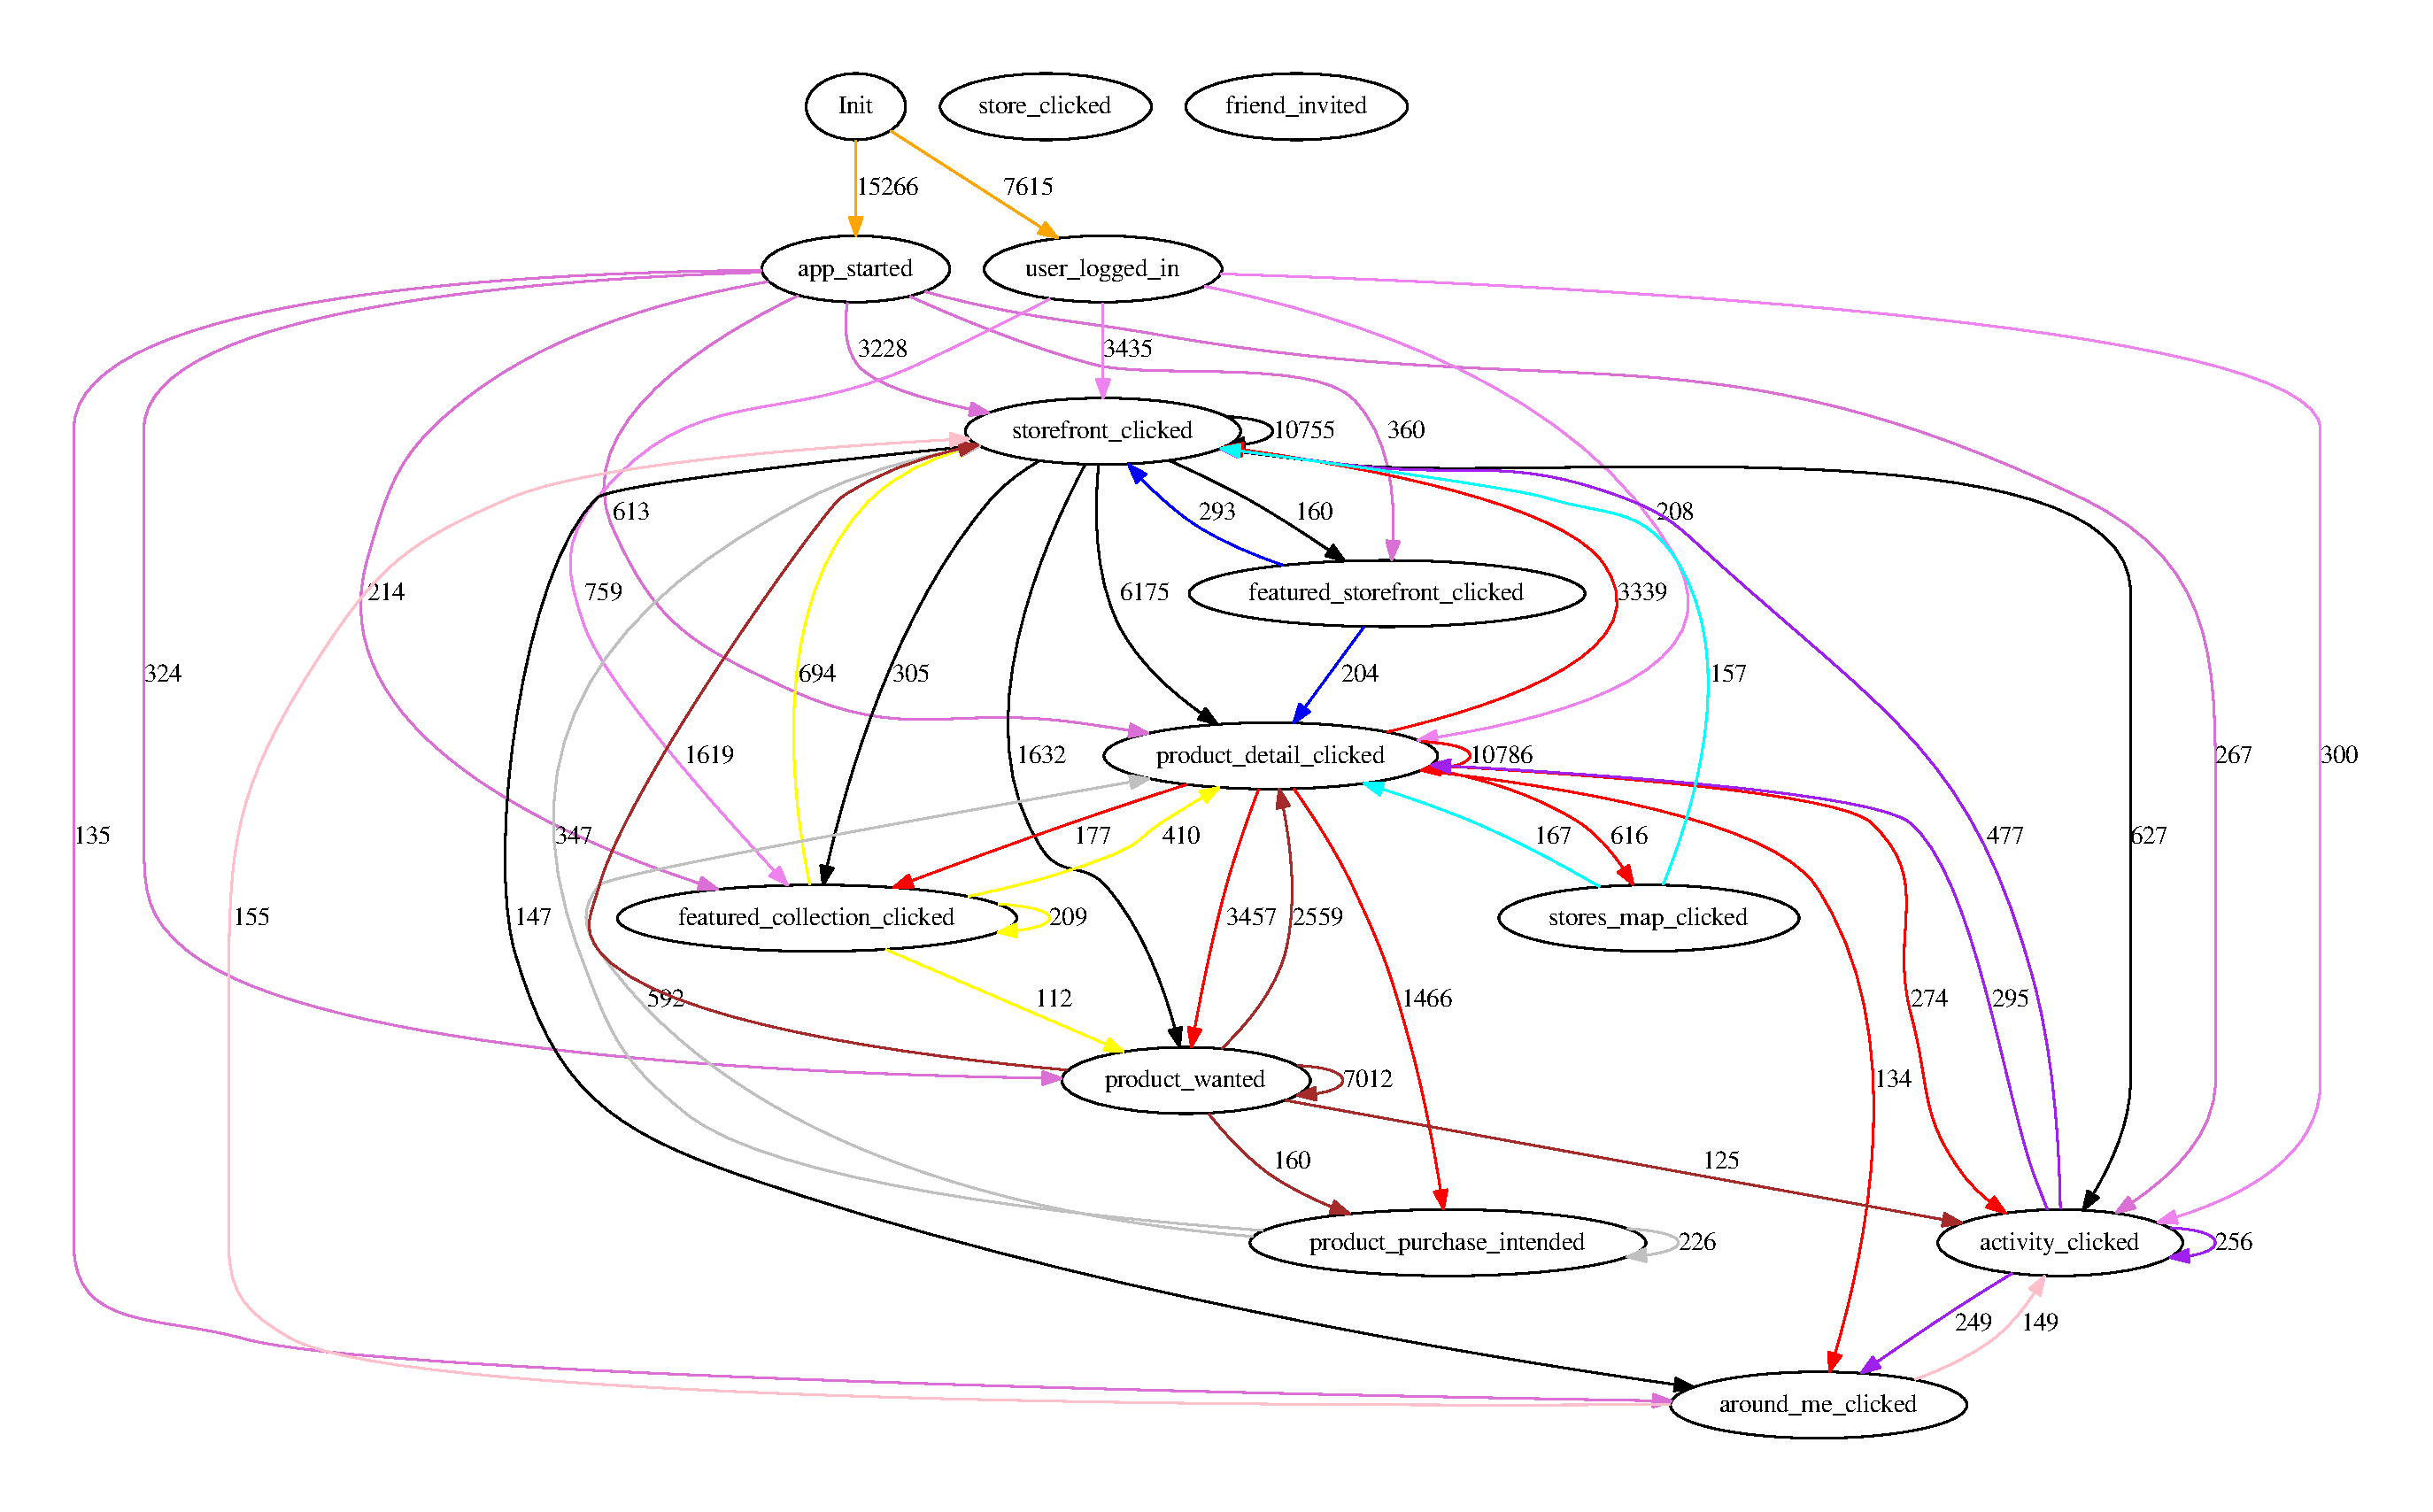
\includegraphics[width=5in]{image/statesInteractionFalse-gvfile.pdf}
        \centering
        \caption[States in session and how they interact]{The different states of the system and how they interact with each other.}
        \label{figure:statesInteractions}
    \end{figure}

\chapter{Extended State Of the Art}
\label{app:sota}

\section{Fashion domain}

\marginpar{TODO: Fix some kind of left align centering og content}
\begin{table}[H]
    \centering
    \begin{tabular}{ccc}
    \toprule
      \multicolumn{2}{c}{Concrete Attributes (Product Features)} & Abstract Attributes (Attitude-Based) \\
      \cmidrule(r{1em}){1-2}
      \multicolumn{1}{c}{Intrinsic (Hedonic)} & \multicolumn{1}{c}{Extrinsic} 				 	& \\ \midrule
      Style 				& Price						 	& Fun \\
      Color				& Brand 					 	& Entertainment \\
      Patten 				& Country of origin			 	& Enjoyment\\
      Fabric/fiber 		& Place(Store) 				 	& Need \\
      Appearance	   	 	& Salespeson's evaluation	 	&  Function\\
      Fashionability  	& Approval of others 		 	&\\
      Durability			& Coordination with wardrobe 	&\\
      Comfort				&								& \\
      Quality				&								& \\
      Fit					&								& \\
      Care 				&								& \\
    \bottomrule
    \end{tabular}
    \caption[Consumers' Purchase Decisions]{The attributes effecting the consumer when in the process of consuming products~\cite{dutton2006}}
    \label{table:ConsumersPurchaseDec}
\end{table}

\section{SoBazaar Competitors}\label{app:sec:soCompetitors}
\subsubsection{Flink} % (fold)
\label{par:flink}
    "Flink is THE brand-new app to discover, get inspired and share trendy looks from top fashion bloggers" - About Flink~\cite{flink}.

    Flink is a fashion discovery application for iPhone.
    It allows the user to browse fashion blogs, hot brands and new trends.

    The content displayed can be "liked" and can be a collection of clothes from different brands.
    If the user is interested in the item, the application can redirect the user to the web page where it is sold.
    \begin{table}[H]
            \centering
            \begin{tabularx}{\linewidth}{>{\parskip1ex}X@{\kern4\tabcolsep}>{\parskip1ex}X}
                \toprule
                \hfil\bfseries Strengths
                &
                \hfil\bfseries Weaknesses
                \\\cmidrule(r{3\tabcolsep}){1-1}\cmidrule(l{-\tabcolsep}){2-2}
                Can follow other users \par
                Connect with facebook \par
                Ability to add item to a \emph{want list} \par
                &
                No personalized recommendations \par
                \\\bottomrule
                \end{tabularx}
        \caption[Recommendation related strengths and weaknesses of Flink~\cite{flink}]{This table is the list of the recommendation related strengths and weaknesses of the mobile fashion application Flink~\cite{flink}}
        \label{table:iphoneAppFlink}
    \end{table}
  % todo - might be more, but can't explore the application since it is iOS 7 required
% paragraph flink (end)

\subsubsection{Motilo} % (fold)
\label{par:motilo}
    "Motilo was launched in 2011 to answer that perennial fashion dilemma all women face -- what shall I wear tonight?" - About Motilo~\cite{motilo}.

    Items on the web page are gathered by the Motilo stylists.
    This gives the page a fresh set of items for the user to select from.

    Motilo gives the user the ability to put together item sets through dragging and dropping the items into a "fashion dilemma", or simply like items.
    The user can ask friends, the Motilo community or the Motilo stylists about suggestions regarding what to wear.
    If the user wants to buy an item, Motilo redirects the user to the page which sells the item in question.

    \begin{table}[H]
    \centering
    \begin{tabularx}{\linewidth}{>{\parskip1ex}X@{\kern4\tabcolsep}>{\parskip1ex}X}
        \toprule
        \hfil\bfseries Strengths
        &
        \hfil\bfseries Weaknesses
            \\\cmidrule(r{3\tabcolsep}){1-1}\cmidrule(l{-\tabcolsep}){2-2}
            Connected with facebook \par
            Ability to add item to a "want list" \par
            A feed with the most trending item collections \par
            Ask Motilo stylists for suggestions \par
            &
            Manual/limited personalized recommendations \par
            \\\bottomrule
            \end{tabularx}
            \caption[Recommendation related strengths and weaknesses of Motilo~\cite{motilo}]{This table is the list of the recommendation related strengths and weaknesses of e-commerce fashion web site Motilo~\cite{motilo}}
            \label{table:ecommenreceMotilo}
        \end{table}
% paragraph motilo (end)


\subsubsection{ModCloth} % (fold)
\label{par:modcloth}
    "A top e-retailer of indie clothing, accessories, and decor, and provide an engaging shopping experience where you, our customer, can have a voice" - About ModCloth~\cite{modcloth}

    ModCloth focuses on giving what the community is looking for.
    The user is given the opportunity to both be the seller and the buyer.
    The item base is affected by the user trough voting.
    \begin{table}[H]
            \centering
            \begin{tabularx}{\linewidth}{>{\parskip1ex}X@{\kern4\tabcolsep}>{\parskip1ex}X}
                \toprule
                \hfil\bfseries Strengths
                &
                \hfil\bfseries Weaknesses
                \\\cmidrule(r{3\tabcolsep}){1-1}\cmidrule(l{-\tabcolsep}){2-2}
                Ability to add item to a "want list" \par
                A feed with the most popular items \par
                A feed with new items \par
                A list of similar items \par
                &
                No personalized recommendations \par
                \\ \bottomrule
        \end{tabularx}
        \caption[Recommendation related strengths and weaknesses of
        ModCloth~\cite{modcloth}]{This table is the list of the recommendation
        related strengths and weaknesses of e-commerce fashion web site
        ModCloth~\cite{modcloth}}
        \label{table:ecommenreceModCloth}
    \end{table}
% paragraph modcloth (end)

\subsubsection{UsTrendy} % (fold)
\label{par:ustrendy}
    "UsTrendy allows you to shop and discover one-of-a-kind fashions from all over the world." - About UsTrendy~\cite{UsTrendy}

    UsTrendy has a large item database of more than hundred thousand unique items.

    When the user is viewing an item, UsTrendy displays other items the user might like, which have common traits with the one the user is currently watching.
    The currently viewed item can be added to a sopping cart.
    \begin{table}[H]
                \centering
                \begin{tabularx}{\linewidth}{>{\parskip1ex}X@{\kern4\tabcolsep}>{\parskip1ex}X}
                    \toprule
                    \hfil\bfseries Strengths
                    &
                    \hfil\bfseries Weaknesses
                    \\\cmidrule(r{3\tabcolsep}){1-1}\cmidrule(l{-\tabcolsep}){2-2}
                  Ability to add item to a "want list" \par
                  A feed with the most popular items \par
                  A feed with new items \par
                  A list of similar items \par
                  &
                  No personalized recommendations \par
                \\ \bottomrule
        \end{tabularx}
        \caption[Recommendation related strengths and weaknesses of UsTrendy~\cite{UsTrendy}]{This table is the list of the recommendation related strengths and weaknesses of e-commerce fashion web site UsTrendy~\cite{UsTrendy}}
        \label{table:ecommenreceUsTrendy}
    \end{table}
% paragraph ustrendy (end)

\subsubsection{Polyvore} % (fold)
\label{par:polyvore}
    "Polyvore is a new way to discover and shop for things you love." - About Polyvore~\cite{polyvore}

    In Polyvore the user can put together sets of items and show them off to their friends and others.
    The items shown on Polyvore are gathered based on the community of Polyvore.

    When accessing an item the user is shown similar items to the one which is currently being watched.
    When the user want to purchase an item, the user is redirected to the page which sells the item.
    \begin{table}[H]
                \centering
                \begin{tabularx}{\linewidth}{>{\parskip1ex}X@{\kern4\tabcolsep}>{\parskip1ex}X}
                \toprule
                \hfil\bfseries Strengths
                &
                \hfil\bfseries Weaknesses
                \\\cmidrule(r{3\tabcolsep}){1-1}\cmidrule(l{-\tabcolsep}){2-2}
                    Ability to add item to a "want list" \par
                    The user can follow other users \par
                    Crawl other fashion sites to add to their item base \par
                    A feed with trending items \par
                    A list of recently viewed items \par
                &
                    No personalized recommendations \par
                \\ \bottomrule
        \end{tabularx}
        \caption[Recommendation related strengths and weaknesses of
        Polyvore~\cite{polyvore}]{This table is the list of the recommendation
        related strengths and weaknesses of e-commerce fashion web site
        Polyvore~\cite{polyvore}}
        \label{table:ecommenrecePolyvore}
    \end{table}
% paragraph polyvore (end)

\subsubsection{Clothia} % (fold)
\label{par:clothia}
    "An online destination where you can mix and match outfits, share looks you love, even try on clothes virtually via your webcam using augmented reality technology" - About Clothia~\cite{clothia}

    The user can put together a set of clothes from the web site and make a "set".
    The set can be shared with other users and like by other users.
    If the user is interested in buying an item, the user is redirected to the page from which the item is sold.
    \begin{table}[H]
                \centering
                \begin{tabularx}{\linewidth}{>{\parskip1ex}X@{\kern4\tabcolsep}>{\parskip1ex}X}
                \toprule
                \hfil\bfseries Strengths
                &
                \hfil\bfseries Weaknesses
                \\\cmidrule(r{3\tabcolsep}){1-1}\cmidrule(l{-\tabcolsep}){2-2}
                Ability to add item to a "want list" \par
                The user can follow other users \par
                A feed with trending items \par
                &
                Lack personalized recommendations \par
                \\ \bottomrule
        \end{tabularx}
        \caption[Recommendation related strengths and weaknesses of Clothia~\cite{clothia}]{This table is the list of the recommendation related strengths and weaknesses of e-commerce fashion web site Clothia~\cite{clothia}}
        \label{table:ecommenreceClothia}
    \end{table}
% paragraph clothia (end)

\subsubsection{Trendabl} % (fold)
\label{par:trendabl}
    "Trendabl is a community of people who love fashion" - About Trendable~\cite{trendabl}

    The user is shown a feed with the newest items, and is free to browse different sets of collections, such as collections with shoes and pants.
    If the user wants to buy an item it can be added to a shopping chart.
    \begin{table}[H]
                    \centering
                    \begin{tabularx}{\linewidth}{>{\parskip1ex}X@{\kern4\tabcolsep}>{\parskip1ex}X}
                    \toprule
                    \hfil\bfseries Strengths
                    &
                    \hfil\bfseries Weaknesses
                    \\\cmidrule(r{3\tabcolsep}){1-1}\cmidrule(l{-\tabcolsep}){2-2}
                    Ability to add item to a "want list" \par
                    The user can follow other users \par
                    System recommends the top users in the system for the user to follow \par
                    &
                    No personalized recommendations \par
                    \\ \bottomrule
        \end{tabularx}
        \caption[Recommendation related strengths and weaknesses of Trendabl~\cite{trendabl}]{This table is the list of the recommendation related strengths and weaknesses of e-commerce fashion web site Trendabl~\cite{trendabl}}
        \label{table:ecommenreceTrendabl}
    \end{table}
% paragraph trendabl (end)


\subsubsection{Rue La La} % (fold)
\label{par:rue_la_la}
    "Rue La La is the destination for the most desired brands" - About Rue La La~\cite{RueLaLa}

    Rue La La is a sale on site e-commerce web site.
    It is built up of a set of different boutiques, which can be browsed by the user.
    When the user is watching an item, Rue La La shows other items from the current boutique.

    \begin{table}[H]
                \centering
                \begin{tabularx}{\linewidth}{>{\parskip1ex}X@{\kern4\tabcolsep}>{\parskip1ex}X}
                \toprule
                \hfil\bfseries Strengths
                &
                \hfil\bfseries Weaknesses
                \\\cmidrule(r{3\tabcolsep}){1-1}\cmidrule(l{-\tabcolsep}){2-2}
                Ability to add item to a "want list" \par
                List of most popular items \par
                &
                No personalized recommendations \par
                \\ \bottomrule
        \end{tabularx}
        \caption[Recommendation related strengths and weaknesses of Rue La La~\cite{RueLaLa}]{This table is the list of the recommendation related strengths and weaknesses of e-commerce fashion web site Rue La La~\cite{RueLaLa}}
        \label{table:ecommenreceRueLaLa}
    \end{table}
% paragraph rue_la_la (end)

\subsubsection{Zalando} % (fold)
\label{par:zalando}
    "Clothes, accessories, sports items, beauty products" - About Zalando~\cite{Zalando}

    Zalando has a large set of items.
    When browsing an item the user is shown a set of similar items the user might also like, and a set of items which might "go well"  with the currently viewed item.

    \begin{table}[H]
                    \centering
                    \begin{tabularx}{\linewidth}{>{\parskip1ex}X@{\kern4\tabcolsep}>{\parskip1ex}X}
                    \toprule
                    \hfil\bfseries Strengths
                    &
                    \hfil\bfseries Weaknesses
                    \\\cmidrule(r{3\tabcolsep}){1-1}\cmidrule(l{-\tabcolsep}){2-2}
                    Ability to add item to a "want list" \par
                    Shop on site \par
                    Similar items \par
                    &
                    No personalized recommendations \par
                    \\ \bottomrule
        \end{tabularx}
        \caption[Recommendation related strengths and weaknesses of Zalando~\cite{Zalando}]{This table is the list of the recommendation related strengths and weaknesses of e-commerce fashion web site Zalando~\cite{Zalando}}
        \label{table:ecommenreceZalando}
    \end{table}
% paragraph zalando (end)

\subsubsection{Ellos~\cite{Ellos}} % (fold)
\label{par:ellos}
    Ellos is a e-commerce web site, which specializes in fashion.

    When browsing an item, similar items to the one currently being watched is presented to the user.
    Other items which might go well with the item is also presented for the user.

    \begin{table}[H]
                \centering
                \begin{tabularx}{\linewidth}{>{\parskip1ex}X@{\kern4\tabcolsep}>{\parskip1ex}X}
                \toprule
                \hfil\bfseries Strengths
                &
                \hfil\bfseries Weaknesses
                \\\cmidrule(r{3\tabcolsep}){1-1}\cmidrule(l{-\tabcolsep}){2-2}
                Ability to add item to a "want list" \par
                Shop on site \par
                Similar items \par
                On site most popular list \par
                Items which might go well with the current \par
                &
                No personalized recommendations \par
                \\ \bottomrule
        \end{tabularx}
        \caption[Recommendation related strengths and weaknesses of Ellos~\cite{Ellos}]{This table is the list of the recommendation related strengths and weaknesses of e-commerce fashion web site Ellos~\cite{Ellos}}
        \label{table:ecommenreceEllos}
    \end{table}
% paragraph ellos (end)

\subsubsection{LookBook} % (fold)
\label{par:lookbook}
    "LOOKBOOK is the \#1 source for fashion inspiration from real people around the world." - About LookBook~\cite{LookBook}

    LookBook is a leading online community which is centered around the looks of the users.
    The users can share their own looks and keep up with other users through watching their uploads.
    With over 1.2 million members LookBook is constantly up to date on the newest fashion trends.
    \begin{table}[H]
                \centering
                \begin{tabularx}{\linewidth}{>{\parskip1ex}X@{\kern4\tabcolsep}>{\parskip1ex}X}
                \toprule
                \hfil\bfseries Strengths
                &
                \hfil\bfseries Weaknesses
                \\\cmidrule(r{3\tabcolsep}){1-1}\cmidrule(l{-\tabcolsep}){2-2}
                Ability to add item to a "want list" \par
                Shop on site \par
                Similar items \par
                Most popular items list \par
                Hot items list \par
                &
                No personalized recommendations \par
                \\ \bottomrule
        \end{tabularx}
        \caption[Recommendation related strengths and weaknesses of LookBook~\cite{LookBook}]{This table is the list of the recommendation related strengths and weaknesses of e-commerce fashion web site LookBook~\cite{LookBook}}
        \label{table:ecommenreceLookBook}
    \end{table}
% paragraph lookbook (end)


\subsubsection{Fashiolista} % (fold)
\label{par:fashiolista}
    "Let Fashiolista's community be your style guide in the online fashion jungle" - About Fasho~\cite{Fashiolista}

    The items on Fashiolista is selected by the users of Fashiolista, and the sites is therefore customized to fit the user crowd's wishes and interests.

    When accessing an item, the user is presented with the item, and a set of other items from the store the current item originated from.
    Other users who liked the item are also shown, so the user can browse their personal want list.
    \begin{table}[H]
                    \centering
                    \begin{tabularx}{\linewidth}{>{\parskip1ex}X@{\kern4\tabcolsep}>{\parskip1ex}X}
                    \toprule
                    \hfil\bfseries Strengths
                    &
                    \hfil\bfseries Weaknesses
                    \\\cmidrule(r{3\tabcolsep}){1-1}\cmidrule(l{-\tabcolsep}){2-2}
                Ability to add item to a "want list" \par
                On site most popular list \par
             &
                 No personalized recommendations \par
             \\ \bottomrule
        \end{tabularx}
        \caption[Recommendation related strengths and weaknesses of Fashiolista~\cite{Fashiolista}]{This table is the list of the recommendation related strengths and weaknesses of e-commerce fashion web site Fashiolista~\cite{Fashiolista}}
        \label{table:ecommenreceFahiolista}
    \end{table}
% paragraph fashiolista (end)

\subsubsection{ShopStyle} % (fold)
\label{par:shopstyle}
    "POPSUGAR is a global women's lifestyle brand focused in media, commerce, and technology" - About ShopStyle~\cite{ShopStyle}

    ShopStyle is a commerce brand of POPSUGAR.
    ShopStyle displays items from other e-commerce web sites, and redirects the user directly to the e-commerce web site from which the item clicked originated.
    Items can be liked on ShopStyle, and viewed in less detail at the web page of ShopStyle.
    \begin{table}[H]
                    \centering
                    \begin{tabularx}{\linewidth}{>{\parskip1ex}X@{\kern4\tabcolsep}>{\parskip1ex}X}
                    \toprule
                    \hfil\bfseries Strengths
                    &
                    \hfil\bfseries Weaknesses
                    \\\cmidrule(r{3\tabcolsep}){1-1}\cmidrule(l{-\tabcolsep}){2-2}
                Ability to add item to a "want list" \par
                Similar items \par
                Editor's picks \par
            &
                No personalized recommendations \par
            \\ \bottomrule
        \end{tabularx}
        \caption[Recommendation related strengths and weaknesses of ShopStyle~\cite{ShopStyle}]{This table is the list of the recommendation related strengths and weaknesses of e-commerce fashion web site ShopStyle~\cite{ShopStyle}}
        \label{table:ecommenreceShopStyle}
    \end{table}
% paragraph shopstyle (end)

\section{Evaluation}
\label{appendix:evaluation-metrics}

% Describe why this is in the Appendix.
In this section we will cover an in-depth study of evaluation metrics and
methods, which were not included in~\ref{sec:evaluation} as they are not
directly suited for either the domain or setting in the proposed system.
They are included here as they may provide clarity on \textit{why} they are not
suited, as well the fact that non-suitednes is a result in itself. Finally we
identify some resources of which the avid reader may do further research into
the field of evaluation recommender systems.

% Boostrapping in Appendix, as we do not use it and Helge proposed it.
\subsubsection{Using bootstrapping for validating offline experiments}
Bootstrapping~\cite{efron1994introduction} is used to estimate properties of an
estimate, such as bias, variance, confidence, intervals and prediction error.
This is done trough measuring these properties when sampling from an
approximated distribution, creating an empirical distribution of the observed
data.  Since the entire population is unknown it will not be possible to
calculate the true error from the sample data.  The idea then is that with this
information from sample data it is possible to say something about the
population.  Since it will not be possible to perform inference on:

\emph{sample data} $\rightarrow$ \emph{population} this is modeled as:
\emph{re-sample data} $\rightarrow$ \emph{sample data}.
The \emph{re-sample data} is a re-sampling of the sample data.

In practice an example to bootstrapping is when we want to calculate the
average height of the population worldwide.  The issue here is that it is not
as doable to measure everyone, so a subset of the population is used.  Since
the average on this number only will be an estimate of the actual world wide
average a sense of error margin must be introduced.  Bootstrapping is then used
to reduce the error of margin through re-sampling the sample data a large
number of times~\footnote{Numbers vary on sample size, but is often 1 000 to 10
000}, and new averages are calculated.  With these averages a histogram can be
produced, which provides an estimate of the distribution of this average.

\begin{figure}[H]
    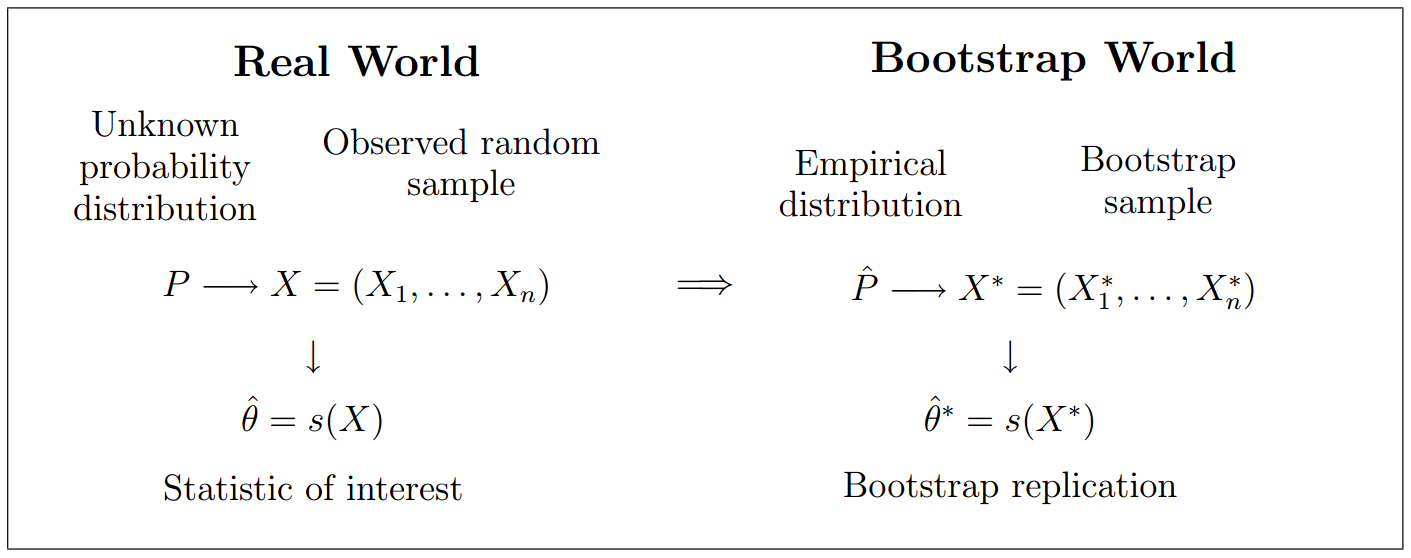
\includegraphics[scale=0.5]{image/bootstrap.png}
    \centering
    \caption[Bootstrapping principles]{A figure of the principles bootstrapping. Taken from~\cite{Eichler2003}}
    \label{figure:bootstrapping}
\end{figure}

One prominent issue with bootstrapping is that important properties of the
actual data might not be caught when undertaking the bootstrapping analysis
~\footnote{"Bootstrapping" comes from the phrase, "to pull oneself up by one's
bootstraps"~\cite{bootstrapSaying1843}}.

% Sub-section on resources available for avid readers who want further research
% into the field of evaluating recommender systems.
\subsubsection{Datasets for Offline Evaluation}
The main aim of a recommender system is to identify the set of items in a
dataset that might be interesting to a user based on their expressed
preferences. For a fashion recommender this would mean estimating how much a
user might like an item, by e.g.\\ predicting what rating a user might give an
item. In recent years, various test collections for different domains such as
books, music, movies have been made available to the public. These datasets
usually consist of user ratings similar to the ones used in this thesis (see
Section~\ref{}):

\begin{table}[H]
\centering
	\begin{tabular}{*{4}l}
	\toprule
		User ID & Item ID & Rating & Timestamp \\ \midrule
		1		  &	11	  &	5	    &  2014-12-15 10:14:51  \\
		2		  &	19	  &	2	    &  2014-12-12 11:44:31  \\
		\dots &	\dots &	\dots &  \dots                \\
	\bottomrule
	\end{tabular}
\caption{Classical recommender system dataset}
\end{table}

In recent years more or more datasets have been made available which contains
additional information such as demographic information about the users,
trust-networks, user-assigned tags and etc. Below we have listed a few selected
popular datasets containing additional information:

\begin{itemize}

\item \textbf{MovieLens 100k dataset}~\cite{Movielens}: The movielens dataset
	incorporates demographic information about the user in addition the
	traditional rating matrix

\item \textbf{Epinions dataset}~\cite{Epinions}: The Epinions dataset includes a
	trust-network, which specifices who-trust-whom in a social network based on
	customer reviews for the website Epinions.com

\item \textbf{The Million Song Dataset}~\cite{Bertin-Mahieux2011}: The million song
	dataset is a implicit feedback dataset. This data also includes information on the users,
	and audio features and song meta-data.

\item \textbf{The Book-Crossing Dataset}: The bookcrossing dataset consists of both implicit and explicit feedback,
	demographic information about users and some content based information about the books.
\end{itemize}

\chapter{Extended Implementation}
\label{app:impl}

\section{Implemented Functional Requirements}
\begin{enumerate}[label=\bfseries FR \arabic*:]
  \item {\color{ForestGreen}Blablaba}
  \item {\color{RedOrange}\st{Blablaba}}
\end{enumerate}

\section{Implemented Non Functional Requirements}
\begin{enumerate}[label=\bfseries NFR \arabic*:]
  \item {\color{ForestGreen}Blablaba}
  \item {\color{RedOrange}\st{Blablaba}}
\end{enumerate}

\section{Experimental Results}
\label{app:results}

\begin{table}[H]
\centering
\resizebox{
\columnwidth}{!}{
\begin{tabular}{*{19}l}
\toprule
Model & AUC &	$MAP@20$ &	$T_{click}$ &	$T_{want}$ &	$T_{purchase}$ &	$P_{click}$&	$P_{want}$ &	$P_{purchase}$ &	$R_{click}$ &	$R_{want}$ &	$R_{purchase}$ &	$MAP@20_{click}$ &	$MAP@20_{want}$	& $MAP@20_{purchase}$ &	 \\
\midrule
\rowcolor{Gray}
Most Popular 			  &	0.627207 &	0.002821 &	1419 &	1280 &	2 &	20 &	10 &	0 &	0.014094 &	0.007812 &	0 &	0.002501 &	0.003635 &	0 &	 \\
ItemBasedKNN k=50     	  &	0.417509 &	0.000404 &	1419 &	1280 &	2 &	4  &	0  &	0 &	0.002819 &	0 		 &	0 &	0.000505 &	0 		 &	0 &	 \\
ItemBasedKNN k=80      	  &	0.490309 &	0.001417 &	1419 &	1280 &	2 &	7  &	8  &	0 &	0.004933 &	0.00625 &	0 &	0.000836 &	0.002755 &	0 &	 \\
UserBasedKNN k=50 	      &	0.496582 &	0.007029 &	1419 &	1280 &	2 &	18 &	11 &	0 &	0.012685 &	0.008594 &	0 &	0.00247 &	0.025629 &	0 &	 \\
ItemBasedKNN k=100  	  & 0.446664 &	0.000376 &	1419 &	1280 &	2 &	4  &	0  &	0 &	0.002819 &	0  		 &	0 &	0.000466 &	0 		 &	0 &	 \\
BPR-MF 			    	  &	0.624658 &	0.001764 &	1419 &	1280 &	2 &	9  &	6  &	0 &	0.006342 &	0.004687 &	0 &	0.001049 &	0.002891 &	0 &	 \\
\bottomrule
\end{tabular}
}
\caption{Appendix: Experimental Results - Time Split 7. May - 19. May}
\end{table}

\begin{table}[H]
\label{appendix:time-based-results}
\centering
\resizebox{
\columnwidth}{!}{
\begin{tabular}{*{19}l}
\toprule
Model & AUC &	$MAP@20$ &	$T_{click}$ &	$T_{want}$ &	$T_{purchase}$ &	$P_{click}$&	$P_{want}$ &	$P_{purchase}$ &	$R_{click}$ &	$R_{want}$ &	$R_{purchase}$ &	$MAP@20_{click}$ &	$MAP@20_{want}$	& $MAP@20_{purchase}$ &	 \\
\midrule
\rowcolor{Gray}
Most Popular 		 		&	0.613218 &	0.004856 &	3038 &	2328 &	36 &	28 &	10 &	0 &	0.009217 &	0.004296 &	0 		 &	0.004622 &	0.003046 &	0 		 &	 \\
ItemBasedKNN k=10 cos		& 	0.362571 &	0.002441 &	3038 &	2328 &	36 &	14 &	13 &	3 &	0.004608 &	0.005584 &	0.083333 &	0.001399 &	0.00248  &	0.051515 &	 \\
ItemBasedKNN jaccard k=50   &	0.418569 &	0.004367 &	3038 &	2328 &	36 &	12 &	9  &	2 &	0.00395  &	0.003866 &	0.055556 &	0.003914 &	0.002017 &	0.014286 &	 \\
ItemBasedKNN jaccard k=100	& 	0.464325 &	0.002638 &	3038 &	2328 &	36 &	14 &	7  &	1 &	0.004608 &	0.003007 &	0.027778 &	0.002576 &	0.000623 &	0.002778 &	 \\
UserBasedKNN k=10			&	0.392918 &	0.002205 &	3038 &	2328 &	36 &	11 &	8  &	3 &	0.003621 &	0.003436 &	0.083333 &	0.000984 &	0.002686 &	0.063582 &	 \\
UserBasedKNN k=50			& 	0.512886 &	0.003248 &	3038 &	2328 &	36 &	14 &	13 &	3 &	0.004608 &	0.005584 &	0.083333 &	0.001766 &	0.005781 &	0.063005 &	 \\
UserBasedKNN k=100			& 	0.558578 &	0.004608 &	3038 &	2328 &	36 &	15 &	15 &	3 &	0.004937 &	0.006443 &	0.083333 &	0.002867 &	0.009185 &	0.069444 &	 \\
UserBasedKNN k=200  		&	0.585442 &	0.004358 &	3038 &	2328 &	36 &	17 &	14 &	3 &	0.005596 &	0.006014 &	0.083333 &	0.002927 &	0.007883 &	0.053241 &	 \\
BPR-MF	 					&	0.601683 &	0.004902 &	3038 &	2328 &	36 &	21.8 &	9 &	  0.8 &	0.007176 &	0.003866 &	0.022222 &	0.004574 &	0.002854 &	0.004762 &	\\
BPR-Linear					&	0.559033 &	0.000443 &	3038 &	2328 &	36 &	2 	&	2 &		0 &	0.000658 &	0.000859 &	0 		 &	0.000136 &	0.000709 &	0 &	\\
Item Average Count			&	0.504619 &	0.000092 &	3038 &	2328 &	36 &	1 &		0 &		0 &	0.000329 &	0 		 &	0 		 &	0.00013  &	0 		 &	0 &	 \\
Item Average Price 			&	0.543423 &	0.000031 &	3038 &	2328 &	36 &	0 &		1 &		0 &	0 		 &	0.00043  &	0 		 &	0 		 &	0.000091 &	0 &	 \\
Item Average Blend 1		&	0.449448 &	0.00469  &	3038 &	2328 &	36 &	14&		17&		0 &	0.004608 &	0.007302 &	0 		 &	0.003783 &	0.003101 &	0 &	 \\
Item Average Popularity 	&	0.379832 &	0.000633 &	3038 &	2328 &	36 &	7 &		8 &		1 &	0.002304 &	0.003436 &	0.027778 &	0.000235 &	0.000999 &	0.000505 &	 \\
Item Average Recentness 	&	0.553508 &	0.000955 &	3038 &	2328 &	36 &	6 &		3 &		0 &	0.001975 &	0.001289 &	0 		 &	0.000861 &	0.00048  &	0 &	 \\
%mahout ItemBased Pearson Correlation
IBCF Count				&	0.421494 &	0.002988 &	3038 &	2328 &	36 &	16 &	5 &		0 &	0.005267 &	0.002148 &	0 		 &	0.002921 &	0.000783 &	0 &	 \\
IBCF Price				&	0.419343 &	0.003714 &	3038 &	2328 &	36 &	18 &	5 &		1 &	0.005925 &	0.002148 &	0.027778 &	0.003313 &	0.001435 &	0.000379 &	 \\
IBCF Blend 1			&	0.420235 &	0.001436 &	3038 &	2328 &	36 &	10 &	7 &		0 &	0.003292 &	0.003007 &	0		 &	0.001231 &	0.001209 &	0 &	 \\
IBCF Popularity			&	0.326705 &	0		 &	3038 &	2328 &	36 &	0  &	0 &		0 &		0 	 &	0		 &	0 		 &	0 		 &	0 		 &	0		 &	 \\
IBCF Recentness			&	0.420134 &	0.002205 &	3038 &	2328 &	36 &	14 &	10&		0 &	0.004608 &	0.004296 &	0 		 &	0.002499 &	0.001059 &	0 &	 \\
%mahout UserBasedKNN k = 50
UserBasedKNN k=50 Count				&	0.402149 &	0.002182 &	3038 &	2328 &	36 &	15 &	7 &		0 &	0.004937 &	0.003007 &	0 		 &	0.001677 &	0.002308 &	0 &	 \\
UserBasedKNN k=50 Price				&	0.395368 &	0.001096 &	3038 &	2328 &	36 &	19 &	5 &		0 &	0.006254 &	0.002148 &	0 		 &	0.000868 &	0.000721 &	0 &	 \\
UserBasedKNN k=50 Blend 1			&	0.394298 &	0.000941 &	3038 &	2328 &	36 &	6  &	3 &		0 &	0.001975 &	0.001289 &	0 		 &	0.00068  &	0.000784 &	0 &	 \\
UserBasedKNN k=50 Popularity 		&	0.405244 &	0.000644 &	3038 &	2328 &	36 &	8  &	5 &		1 &	0.002633 &	0.002148 &	0.027778 &	0.000367 &	0.000558 &	0.002525 &	 \\
UserBasedKNN k=50 Recentness 		&	0.39173  &	0.00109 &	3038 &	2328 &	36 &	8  &	5 &		0 &	0.002633 &	0.002148 &	0 		 &	0.000735 &	0.001022 &	0 &	 \\
%mahout UserBasedKNN k = 100
UserBasedKNN k=100 Count Sigmoid  	&	0.424043 &	0.001937 &	3038 &	2328 &	36 &	11 &	8  &	0 &	0.003621 &	0.003436 &	0 &	0.001601 &	0.002075 &	0 &	 \\
UserBasedKNN k=100 Count Linear  	&	0.422888 &	0.001974 &	3038 &	2328 &	36 &	11 &	5  &	0 &	0.003621 &	0.002148 &	0 &	0.001634 &	0.002172 &	0 &	 \\
UserBasedKNN k=100 Blend  			&	0.424437 &	0.002044 &	3038 &	2328 &	36 &	11 &	10 &	1 &	0.003621 &	0.004296 &	0.027778 &	0.001584 &	0.002733 &	0.000379 &	 \\
UserBasedKNN k=100 Popularity   &	0.406156 &	0.000916 &	3038 &	2328 &	36 &	7  &	9  &	0 &	0.002304 &	0.003866 &	0 &	0.000468 &	0.001349 &	0 &	 \\
UserBasedKNN k=100 Recentness   &	0.406574 &	0.000897 &	3038 &	2328 &	36 &	9  &	7  &	0 &	0.002962 &	0.003007 &	0 &	0.000575 &	0.001153 &	0 &	 \\
%ALSWR 100, 100, 15 true, 10
ALS-WR Count Linear        &   0.628547 &  0.006958 &  3037 &  2328 &  36 & 19.25 & 22.25 & 	3 & 0.006338 &  0.009558 &  0.083333 &  0.005049 &  0.009524 &  0.062978 &   \\
ALS-WR Popularity Linear   &   0.625682 &  0.001705 &  3037 &  2328 &  36 & 13.5  & 12.75 & 	3 & 0.004445 &  0.005477 &  0.083333 &  0.000739 &  0.003915 &  0.014694 &   \\
ALS-WR Blend               &   0.623146 &  0.005666 &  3037 &  2328 &  36 & 19.25 & 14.5  &  	3 & 0.006338 &  0.006229 &  0.083333 &  0.004144 &  0.007086 &  0.059737 &   \\
ALS-WR Recentness Linear   &   0.631948 &  0.006444 &  3037 &  2328 &  36 & 19    & 17.5  & 	3 & 0.006256 &  0.007517 &  0.083333 &  0.004529 &  0.010394 &  0.073505 &   \\
ALS-WR Price Linear        &   0.611358 &  0.003687 &  3037 &  2328 &  36 & 18.75 & 13    &    4 & 0.006174 &  0.005584 &  0.111111 &  0.002123 &  0.007305 &  0.038556 &   \\
\bottomrule
\end{tabular}
}
\caption{Appendix: Experimental Results - Time Split 16. April - 19. May}
\end{table}


\subsubsection{Random Splits}
\label{appendix-random-split-results}
\begin{table}[H]
\centering
\resizebox{
\columnwidth}{!}{
\begin{tabular}{*{19}l}
\toprule
Model & AUC &	$MAP@20$ &	$T_{click}$ &	$T_{want}$ &	$T_{purchase}$ &	$P_{click}$&	$T_{want}$ &	$T_{purchase}$ &	$R_{click}$ &	$R_{want}$ &	$R_{purchase}$ &	$MAP@20_{click}$ &	$MAP@20_{want}$	& $MAP@20_{purchase}$ &	 \\
\midrule
Most-Popular    	&  0.751516     & 0.013236  &   1323    &   1235    &   135     &   63      &   40.75   & 3.5     &   0.0476135   &   0.03300275  &   0.0270445   &   0.0147725   & 0.0111475 &   0.0098995 & \\
ItemBasedLog	   	&  0.690723     & 0.002094  &   1353.9  &   1250.5  &   138     &   8.8     &   4.6     & 1.47    &   0.006488    &   0.003672    &   0.007252    &   0.001470    & 0.002043  &   0.000618  & \\
ItemBasedKNN k=10	&  0.704103     & 0.0199615 &   1332.8  &   1233.8  &   135.4   &   68.9    &   92.4    & 8.4     &   0.0516662   &   0.0748659   &   0.0624243   &   0.0141642   & 0.0287664 &   0.0191711 & \\
ItemBasedKNN k=50	&  0.727482     & 0.0133356 &   1366    &   1264.8  &   141     &   59      &   82.6    & 9.6     &   0.0431518   &   0.0653024   &   0.0675468   &   0.008712    & 0.0184392 &   0.0159292 & \\
ItemBasedKNN k=80   &  0.6923396	& 0.0023332	&	1292.8  & 	1188.6& 	136.6	&	10.2	&	19		& 2.6	  &	0.0078848	&	0.0159932	&	0.094176	&	0.005756	&	0.018417	&	0.0019042	& \\
ItemBasedKNN k=120  &  0.7357796    & 0.0069094 &   1295.8  &   1231.4  &   146.8   & 	37.6    &   53      & 7.2     &   0.0290256   &  0.0431066    &  0.0487262    &  0.0044356    &  0.0097038&   0.0060544 & \\
ItemBasedKnn k=200  &  0.7032954	& 0.0017026	&	1318.4	&   1248.4	&   142.4	&	8.4		&	10.4	& 1.2	  &	  0.0063506	  &	0.0083276	&	0.044265	&	0.008208	&	0.009611	&	0.000862	&	\\
UserKNN K = 10 cos  &  0.6962484	& 0.019008	&	1324.6	&   1227.4 & 	137		&	55.2	&	76		& 9	  	  &	  0.0416912	  &	0.0619346	&	0.327716	&	0.070403	&	0.124173	&	0.0217902	&	\\
UserKNN K = 50 cos  &  0.7596092	& 0.0340278	&	1316.2	&   1233.8 &	142		&	102.4	&	111.2	& 13	  &	  0.077734	  &	0.0901368	&	0.457994	&	0.137837	&	0.202344	&	0.0299614	&	\\
UserKNN K = 80 cos  &  0.781408		& 0.0330702	&	1347.6	&   1199.8 &	140.6	&	101.2	&	115.2	& 12.6    &	  0.0750486	  &	0.0960048	&	0.448823	&	0.128239	&	0.208182	&	0.0248482	&	\\
UserKNN K = 120 cos &  0.7914806	& 0.0325814	&	1287.2	&   1256.4 &	137.4	&	92.6	&	113.4	& 13.2    &	  0.0719976	  &	0.090211	&	0.478547	&	0.128197	&	0.205397	&	0.0289208	&	\\
UserKNN K = 200 cos &  0.7926842	& 0.0317002	&	1282.2	&   1186.2 &	136.4	&	102.2	&	101.4	& 12.6    &	  0.0797042	  &	0.0854958	&	0.471684	&	0.128002	&	0.182436	&	0.0349802	&	\\
BPR-MF          	&  0.7286434    & 0.0099586 &   1332.8  &   1233.8  &   135.4   &   51.4    &   31      & 5.2     &   0.0385224   &   0.025142    &   0.0385042   &   0.0120152   & 0.0058942 &   0.0133786 && \\
BPRLinear       	&  0.7097516    & 0.0070648 &   1344.3  &   1241.9  &   141.3   &   27.4    &   25.1    & 2.5     &   0.0203941   &   0.0202133   &   0.017821    &   0.006298    & 0.0075964 &   0.0022692 & \\
%Itembased average pearson
IBCF Count		&	0.681723 &	0.002987 &	1342.4 &	1244.3 &	128.3 	&	18.8   &	12.9  &	2.9		 &	0.014021 &	0.010418 &	0.024101 &	0.003002 &	0.002092 &	0.002761 &	 \\
IBCF Price		&	0.680758 &	0.004616 &	1332.8 &	1245.7 &	137.15  &	21.1   &	17.6  &	5.63     &	0.015859 &	0.014138 &	0.041189 &	0.003722 &	0.005    &	0.008681 &	 \\
IBCF Blend 1	&	0.684902 &	0.004669 &	1313.5 &	1257.5 &	144 	&	21.7   &	23.2  &	4.25     &	0.016495 &	0.018412 &	0.029243 &	0.004835 &	0.003413 &	0.005781 &	 \\
IBCF Popularity	&	0.554495 &	0.001209 &	1335.7 &	1230.1 &	149.9 	&	0.3    &	6 	  &	5.95     &	0.000198 &	0.004871 &	0.038575 &	0.000028 &	0.002344 &	0.006537 &	 \\
IBCF Recentness	&	0.681045 &	0.00349 &	1300.8 &	1262.9 &	140.8   &	19.9   &	16	  &	3.34     &	0.015231 &	0.012658 &	0.02335 &	0.003443 &	0.002389 &	0.006446 &	 \\

%Userbased average K = 50
UserBasedKNN k=50 Count linear		&	0.6662 	 &	0.003508 &	1334.3 & 	1260.9 &	141.3  &	17.8   &	16.7  &	1.7  &	0.0133   &	0.013211 &	0.012425 &	0.002887 &	0.004206 &	0.002634 &	 \\
UserBasedKNN k=50 Price linear		&	0.657162 &	0.003731 &	1334.7 & 	1268   &	141    &	16 	   &	23.7  &	0.6  &	0.011943 &	0.018701 &	0.004606 &	0.00304 &	0.005287 &	0.000543 &	 \\
UserBasedKNN k=50 Blend 1			&	0.657548 &	0.003138 &	1336.5 & 	1255.8 &	144.2  &	11.7   &	12.1  &	2.5  &	0.008752 &	0.009632 &	0.017344 &	0.003187 &	0.001709 &	0.003402 &	 \\
UserBasedKNN k=50 Popularity Linear	&	0.662589 &	0.00196  &	1329.9 & 	1266.5 &	140.1  &	8.8    &	14    &	1.9  &	0.006632 &	0.010978 &	0.013628 &	0.001192 &	0.002801 &	0.001197 &	 \\
UserBasedKNN k=50 Recentness linear	&	0.630218 &	0.002542 &	1341.7 & 	1248.9	&	153.1  &	14.7   &	12.9  &	3.8  &	0.01     &	0.010284 &	0.025173 &	0.001919 &	0.003005 &	0.002768 &	 \\

%ALS-WR 100 100 15 true 10
ALS-WR Count 		&	0.813701 & 0.032043	&	1340.8	&	1246.6	&	141.9	&	114.4	&	114.5	&	13.2	&	0.085293	&	0.091838	&	0.093449	&	0.027457	&	0.033701	&	0.037635 &	\\
ALS-WR Price		&	0.797892 & 0.034154	&	1340.5	&	1250.8	&	138.0	&	108.3	&	121.4	&	15.0	&	0.080842	&	0.09701		&	0.108833	&	0.028443	&	0.035474	&	0.033493 & 	\\
ALS-WR Blend 1	    &   0.807673 & 0.034147	&	1339.7	&	1255.1	&	134.4	&	117.0	&	125.0	&	12.4	&	0.087277	&	0.099575	&	0.092396	&	0.028199	&	0.041825	&	0.029776 &	\\
ALS-WR Popularity 	&	0.80708	 & 0.023619  &	1332.1	&	1251.2	&	145.9	&	83.0	&	93.6	&	9.7		&	0.062324	&	0.074848	&	0.066325	&	0.018547	&	0.029953	&	0.01606	 &	\\
ALS-WR Recentness	&	0.812053 & 0.037945	&	1337.9	&	1254.5	&	136.8	&	120.8	&	130.2	&	13.5	&	0.090251	&	0.103819	&	0.100385	&	0.031089	&	0.041618	&	0.03764	 &  \\
ALS-WR Blend 2		&	0.800422 &	0.034519 &	1344.75 &	1246.5  &	134.5 &	104.5 		&	120.75 &	13.5 &	0.077686 &	0.097038 &	0.100486 &	0.026307 &	0.041865 &	0.025649 &	 \\
\bottomrule
\end{tabular}
}
\caption{Appendix: Experimental Results - Random Splits}
\end{table}





It was interesting to see that the performance of ItemBasedKNN actually started to decrease when looking at more than 50 neighbors, while UserBasedKNN's performance kept going up or stayed mostly the same when adding
neighbors. UserBasedKNN with between 50-200 neighbors seem to give the best recommendation quality of all the methods tested, and they different is fairly significant.


\begin{table}
\centering\resizebox
{\columnwidth}{!}{
\begin{tabular}{*{19}l}
\toprule
& AUC &	MAP@20 &	T\_c &	T\_w &	T\_p &	P\_c &	P\_w &	P\_p &	R\_c &	R\_w &	R\_p &	MAP@20-click &	MAP@20-want &	MAP@20-purchase &	 \\
\midrule
%Most Popular
item-10 &	0.2964 &	0 &	3241 &	2620.5 &	243 &	0 &	0 &	0 &	0 &	0 &	0 &	0 &	0 &	0 &	 \\
item-75 &	0.973461 &	0.043607 &	989.5 &	712 &	52.5 &	148 &	83 &	6 &	0.149551 &	0.116645 &	0.114296 &	0.050583 &	0.029793 &	0.064658 &	 \\
system-40 &	0.619492 &	0.005504 &	3048 &	2308 &	36 &	29 &	15 &	1 &	0.009514 &	0.006499 &	0.027778 &	0.005144 &	0.003966 &	0.005208 &	 \\
system-80 &	0.601734 &	0.003103 &	3048 &	2308 &	36 &	19 &	11 &	0 &	0.006234 &	0.004766 &	0 &	0.002911 &	0.002184 &	0 &	 \\
system-60 &	0.593922 &	0.004694 &	3048 &	2308 &	36 &	22 &	14 &	0 &	0.007218 &	0.006066 &	0 &	0.004547 &	0.003213 &	0 &	 \\
item-40 &	0.908403 &	0.015807 &	2221 &	1699.5 &	152.5 &	271.5 &	142.5 &	13 &	0.122245 &	0.083855 &	0.085254 &	0.018698 &	0.01177 &	0.013565 &	 \\
user-75 &	0.657664 &	0.005375 &	1000.5 &	1216 &	96 &	18 &	27 &	3.5 &	0.018463 &	0.021551 &	0.04188 &	0.00594 &	0.004096 &	0.00596 &	 \\
user-10 &	0.653873 &	0.017394 &	3673 &	4180.5 &	336.5 &	82 &	90 &	8 &	0.023064 &	0.020592 &	0.023878 &	0.009412 &	0.009061 &	0.007878 &	 \\
user-40 &	0.658753 &	0.010465 &	2416 &	2844.5 &	216.5 &	43 &	62.5 &	9 &	0.01834 &	0.021091 &	0.041581 &	0.006525 &	0.006448 &	0.009125 &	 \\

%SVD
item-10 &	0.548427 &	0.000192 &	3241 &	2620.5 &	243 &	3 &	1 &	0 &	0.000926 &	0.000382 &	0 &	0.000216 &	0.000047 &	0 &	 \\
item-40 &	0.728263 &	0.011774 &	2221 &	1699.5 &	152.5 &	84 &	63 &	4 &	0.037826 &	0.03708 &	0.026232 &	0.010776 &	0.014745 &	0.005461 &	 \\
system-40 &	0.600738 &	0.006208 &	3048 &	2308 &	36 &	13 &	11 &	0 &	0.004265 &	0.004766 &	0 &	0.005055 &	0.014151 &	0 &	 \\
system-80 &	0.570946 &	0.002545 &	3048 &	2308 &	36 &	12 &	8 &	1 &	0.003937 &	0.003466 &	0.027778 &	0.001969 &	0.002149 &	0.041667 &	 \\
system-60 &	0.568137 &	0.001761 &	3048 &	2308 &	36 &	8 &	12 &	1 &	0.002625 &	0.005199 &	0.027778 &	0.00108 &	0.008555 &	0.004167 &	 \\
item-75 &	0.808723 &	0.037148 &	989.5 &	712 &	52.5 &	91.5 &	77.5 &	5 &	0.092468 &	0.108875 &	0.095247 &	0.031812 &	0.040076 &	0.019101 &	 \\
user-75 &	0.747457 &	0.012256 &	1000.5 &	1216 &	96 &	24.5 &	38 &	2 &	0.024894 &	0.030244 &	0.024274 &	0.009066 &	0.016027 &	0.02484 &	 \\
user-10 &	0.669121 &	0.021574 &	3673 &	4180.5 &	336.5 &	56.5 &	82 &	12 &	0.015861 &	0.018796 &	0.035962 &	0.009461 &	0.013781 &	0.020946 &	 \\
user-40 &	0.71492 &	0.015096 &	2416 &	2844.5 &	216.5 &	40.5 &	71 &	8.5 &	0.017286 &	0.024057 &	0.039299 &	0.00768 &	0.012863 &	0.015004 &	 \\
avgs	 &	0.661859 &	0.012061 &	2520.555556 &	2244.111111 &	133.888889 &	37 &	40.388889 &	3.722222 &	0.022232 &	0.025874 &	0.03073 &	0.008568 &	0.013599 &	0.014576 &	\\

%Item-Based
item-10 &	0.581572 &	0.000183 &	3241 &	2620.5 &	243 &	3 &	4 &	0 &	0.000926 &	0.001526 &	0 &	0.000168 &	0.000166 &	0 &	 \\
item-40 &	0.647155 &	0.002948 &	2221 &	1699.5 &	152.5 &	31 &	26 &	2 &	0.01396 &	0.015304 &	0.013116 &	0.002202 &	0.004557 &	0.000428 &	 \\
system-40 &	0.337922 &	0.000842 &	3048 &	2308 &	36 &	7 &	5 &	1 &	0.002297 &	0.002166 &	0.027778 &	0.000625 &	0.001511 &	0.00463 &	 \\
system-80 &	0.344166 &	0 &	3048 &	2308 &	36 &	0 &	0 &	0 &	0 &	0 &	0 &	0 &	0 &	0 &	 \\
system-60 &	0.340169 &	0.00055 &	3048 &	2308 &	36 &	0 &	3 &	0 &	0 &	0.0013 &	0 &	0 &	0.003669 &	0 &	 \\
item-75 &	0.783782 &	0.008705 &	989.5 &	712 &	52.5 &	21 &	13 &	4 &	0.021223 &	0.018261 &	0.076197 &	0.008209 &	0.00558 &	0.026017 &	 \\
user-75 &	0.618759 &	0.003454 &	1000.5 &	1216 &	96 &	1.5 &	11.5 &	1.5 &	0.001534 &	0.009157 &	0.017607 &	0.000947 &	0.004815 &	0.004309 &	 \\
user-10 &	0.525182 &	0.013867 &	3673 &	4180.5 &	336.5 &	29 &	56.5 &	9 &	0.00811 &	0.013058 &	0.026996 &	0.004283 &	0.009368 &	0.012624 &	 \\
user-40 &	0.569436 &	0.005097 &	2416 &	2844.5 &	216.5 &	24 &	34.5 &	4 &	0.010209 &	0.011673 &	0.018497 &	0.003462 &	0.004267 &	0.003834 &	 \\

%SVD 0 0 1 0 1
item-10 &	0.625073 &	0.000518 &	3322.5 &	2617 &	248 &	5 &	7.5 &	0 &	0.001505 &	0.002867 &	0 &	0.000437 &	0.000596 &	0 &	 \\
item-40 &	0.727069 &	0.013534 &	2278 &	1696.5 &	155 &	89.5 &	76.5 &	6 &	0.039285 &	0.045097 &	0.038716 &	0.014394 &	0.015436 &	0.009411 &	 \\
system-40 &	0.617729 &	0.003569 &	3048 &	2308 &	36 &	16 &	12 &	0 &	0.005249 &	0.005199 &	0 &	0.00294 &	0.003113 &	0 &	 \\
system-80 &	0.576757 &	0.001443 &	3048 &	2308 &	36 &	9 &	7 &	0 &	0.002953 &	0.003033 &	0 &	0.001139 &	0.001161 &	0 &	 \\
system-60 &	0.570766 &	0.002491 &	3048 &	2308 &	36 &	11 &	14 &	1 &	0.003609 &	0.006066 &	0.027778 &	0.001242 &	0.004649 &	0.005682 &	 \\
item-75 &	0.785433 &	0.036564 &	1011.5 &	711.5 &	55 &	98 &	80 &	6 &	0.096876 &	0.112471 &	0.109127 &	0.033223 &	0.035562 &	0.043011 &	 \\
user-75 &	0.737931 &	0.011515 &	1094 &	1327.5 &	91 &	25 &	34.5 &	3 &	0.022635 &	0.025434 &	0.030601 &	0.007306 &	0.011666 &	0.00666 &	 \\
user-10 &	0.672386 &	0.028034 &	3952 &	4562.5 &	391 &	65 &	83 &	17.5 &	0.016251 &	0.0179 &	0.041984 &	0.014275 &	0.016082 &	0.022662 &	 \\
user-40 &	0.707324 &	0.016305 &	2609 &	3131 &	218 &	39 &	62.5 &	9 &	0.014753 &	0.019615 &	0.03672 &	0.005155 &	0.017507 &	0.019089 &	 \\

%Itembased 0 0 1 0 1
item-10 &	0.558101 &	0.000614 &	3322.5 &	2617 &	248 &	11 &	5 &	1 &	0.003311 &	0.001911 &	0.004033 &	0.000548 &	0.000845 &	0.000313 &	 \\
item-40 &	0.758747 &	0.002795 &	2278 &	1696.5 &	155 &	23.5 &	11 &	3 &	0.010315 &	0.006484 &	0.019358 &	0.001654 &	0.004507 &	0.00173 &	 \\
system-40 &	0.410766 &	0.000645 &	3048 &	2308 &	36 &	12 &	3 &	0 &	0.003937 &	0.0013 &	0 &	0.000897 &	0.000154 &	0 &	 \\
system-80 &	0.330608 &	0.000442 &	3048 &	2308 &	36 &	2 &	6 &	0 &	0.000656 &	0.0026 &	0 &	0.000151 &	0.000805 &	0 &	 \\
system-60 &	0.360732 &	0.000567 &	3048 &	2308 &	36 &	3 &	7 &	1 &	0.000984 &	0.003033 &	0.027778 &	0.000153 &	0.003944 &	0.004545 &	 \\
item-75 &	0.78616 &	0.00437 &	1011.5 &	711.5 &	55 &	15.5 &	6.5 &	0 &	0.015321 &	0.009145 &	0 &	0.005092 &	0.003701 &	0 &	 \\
user-75 &	0.66947 &	0.000629 &	1094 &	1327.5 &	91 &	1.5 &	2.5 &	0 &	0.001355 &	0.001868 &	0 &	0.000213 &	0.000751 &	0 &	 \\
user-10 &	0.587419 &	0.016058 &	3952 &	4562.5 &	391 &	26 &	58.5 &	13 &	0.006526 &	0.012636 &	0.030767 &	0.009858 &	0.010059 &	0.013228 &	 \\
user-40 &	0.659185 &	0.003011 &	2609 &	3131 &	218 &	7 &	19.5 &	1.5 &	0.00264 &	0.006135 &	0.005515 &	0.000622 &	0.003465 &	0.000174 &	 \\
avgs	 &	0.569021 &	0.003237 &	2601.222222 &	2330 &	140.666667 &	11.277778 &	13.222222 &	2.166667 &	0.005005 &	0.005012 &	0.009717 &	0.002132 &	0.003137 &	0.002221 &	\\

%SVD 0 0 0 0 1
item-10 &	0.585388 &	0 &	3254.5 &	2642.5 &	243.5 &	0 &	0 &	0 &	0 &	0 &	0 &	0 &	0 &	0 &	 \\
item-40 &	0.802813 &	0.014429 &	2232.5 &	1712 &	153.5 &	83 &	67 &	7 &	0.037112 &	0.03914 &	0.045603 &	0.013901 &	0.017344 &	0.011495 &	 \\
system-40 &	0.632071 &	0.003087 &	3048 &	2308 &	36 &	21 &	12 &	0 &	0.00689 &	0.005199 &	0 &	0.002526 &	0.00312 &	0 &	 \\
system-80 &	0.573326 &	0.00213 &	3048 &	2308 &	36 &	20 &	3 &	0 &	0.006562 &	0.0013 &	0 &	0.003496 &	0.000229 &	0 &	 \\
system-60 &	0.582566 &	0.003647 &	3048 &	2308 &	36 &	19 &	5 &	0 &	0.006234 &	0.002166 &	0 &	0.003663 &	0.000609 &	0 &	 \\
item-75 &	0.883175 &	0.028139 &	989 &	722.5 &	54 &	111 &	96 &	5 &	0.112164 &	0.132859 &	0.092624 &	0.028001 &	0.034219 &	0.016794 &	 \\
user-75 &	0.802479 &	0.013645 &	938.5 &	1453.5 &	90.5 &	23.5 &	47 &	4.5 &	0.024681 &	0.03131 &	0.057392 &	0.009095 &	0.018635 &	0.066871 &	 \\
user-10 &	0.750818 &	0.032507 &	3367 &	5001.5 &	418.5 &	68 &	115.5 &	19 &	0.019687 &	0.02235 &	0.045516 &	0.01533 &	0.017845 &	0.035992 &	 \\
user-40 &	0.776184 &	0.021176 &	2213.5 &	3416.5 &	249 &	42 &	89 &	12 &	0.018529 &	0.025151 &	0.049708 &	0.008662 &	0.015711 &	0.046424 &	 \\
avgs	 &	0.709869 &	0.013196 &	2459.888889 &	2430.277778 &	146.333333 &	43.055556 &	48.277778 &	5.277778 &	0.025762 &	0.028831 &	0.032316 &	0.009408 &	0.011968 &	0.019731 &	\\

%Itembased 0 0 0 0 1
item-10 &	0.596502 &	0.0015 &	3254.5 &	2642.5 &	243.5 &	12 &	6 &	1 &	0.003688 &	0.002271 &	0.004107 &	0.001569 &	0.000812 &	0.000098 &	 \\
item-40 &	0.6813 &	0.003662 &	2232.5 &	1712 &	153.5 &	29 &	15 &	3 &	0.012979 &	0.008763 &	0.019544 &	0.003952 &	0.001496 &	0.001828 &	 \\
system-40 &	0.362105 &	0.001836 &	3048 &	2308 &	36 &	14 &	5 &	0 &	0.004593 &	0.002166 &	0 &	0.001767 &	0.001603 &	0 &	 \\
system-80 &	0.328139 &	0.000348 &	3048 &	2308 &	36 &	2 &	1 &	0 &	0.000656 &	0.000433 &	0 &	0.000362 &	0.000034 &	0 &	 \\
system-60 &	0.333955 &	0.002444 &	3048 &	2308 &	36 &	1 &	5 &	1 &	0.000328 &	0.002166 &	0.027778 &	0.000025 &	0.007962 &	0.083333 &	 \\
item-75 &	0.801234 &	0.006053 &	989 &	722.5 &	54 &	22 &	12 &	2 &	0.022237 &	0.016609 &	0.03705 &	0.004121 &	0.002033 &	0.026319 &	 \\
user-75 &	0.642857 &	0.001959 &	938.5 &	1453.5 &	90.5 &	6 &	7.5 &	1.5 &	0.006354 &	0.005027 &	0.019131 &	0.002697 &	0.001044 &	0.000951 &	 \\
user-10 &	0.541997 &	0.014604 &	3367 &	5001.5 &	418.5 &	32 &	58 &	4 &	0.009187 &	0.01123 &	0.009601 &	0.007049 &	0.01106 &	0.004802 &	 \\
user-40 &	0.58478 &	0.005501 &	2213.5 &	3416.5 &	249 &	20.5 &	32.5 &	2 &	0.009037 &	0.009327 &	0.008387 &	0.003424 &	0.005499 &	0.002127 &	 \\
avgs	 &	0.54143 &	0.004212 &	2459.888889 &	2430.277778 &	146.333333 &	15.388889 &	15.777778 &	1.611111 &	0.007673 &	0.006444 &	0.013955 &	0.002774 &	0.003505 &	0.013273 &	\\

\bottomrule
\end{tabular}
}
\caption{Appendix: Cold-start - Time-Based Splits}
\end{table}


\begin{table}
\centering\resizebox
{\columnwidth}{!}{
\begin{tabular}{*{19}l}
\toprule
& AUC &	MAP@20 &	T\_c &	T\_w &	T\_p &	P\_c &	P\_w &	P\_p &	R\_c &	R\_w &	R\_p &	MAP@20-click &	MAP@20-want &	MAP@20-purchase &	 \\
\midrule

%Most Popular - Avg
item-10		&	0.3096225	&	0			&	3256.25	&	2639	&	251	&	0	&	0	&	0	&	0	&	0	&	0	&	0	&	0		0	&	\\
item-40		&	0.90448		&	0.0267585	&	2162.3	&	1778.25	&	161.7	&	261.4	&	166.1	&	13.5	&	0.1207895	&	0.093357	&	0.08314335	&	0.03096785	&	0.01779265	&	0.020967	&	\\
item-75		&	0.8469825	&	0.0234215	&	937.7	&	755.9	&	73.34	&	88.6	&	59.67	&	5.4	&	0.0943945	&	0.07894715	&	0.07447935	&	0.0279395	&	0.0167885	&	0.016906	&	\\
system-40	&	0.663937	&	0.0139605	&	2647.4	&	2469.4	&	277.71	&	88.96	&	72.7	&	6.1	&	0.033597	&	0.029427	&	0.021974	&	0.014782	&	0.01133735	&	0.01091415	&	\\
system-60	&	0.6752165	&	0.0125785	&	2647.4	&	2469.4	&	277.71	&	98.1	&	73.46	&	6.75	&	0.0370545	&	0.0297455	&	0.0243725	&	0.01351435	&	0.00959285	&	0.00799365	&	\\
system-80	&	0.708515	&	0.014044	&	2650	&	2464.9	&	279.6	&	110	&	79.25	&	8.1	&	0.041488	&	0.03214465	&	0.02887465	&	0.01523865	&	0.01043815	&	0.00935215	&	\\
user-10		&	0.7206055	&	0.029688	&	3635.2	&	4493.5	&	389.9	&	142.3	&	122.3	&	10.25	&	0.039089	&	0.02732585	&	0.02675	&	0.0236955	&	0.01601815	&	0.00851165	&	\\
user-40		&	0.7260445	&	0.017628	&	2435.1	&	2997.75	&	263.3	&	89.25	&	81.92	&	6.25	&	0.03653	&	0.02744665	&	0.02343615	&	0.016989	&	0.0114675	&	0.0073835	&	\\
user-75		&	0.729684	&	0.0062015	&	1020.2	&	1279.2	&	107.5	&	22.25	&	22.17	&	1.17	&	0.021841	&	0.01734265	&	0.01177485	&	0.007437	&	0.00359915	&	0.00549415	&	\\

%mahout - itembased - Avg
item-10		&	0.585499	&	0.000022	&	3265.5	&	2650.5	&	251	&	1	&	0.5	&	0	&	0.0003075	&	0.000188	&	0	&	0.000079	&	0.0000115	&	0	&	\\
item-40		&	0.660409	&	0.00571		&	2175	&	1765.5	&	176	&	42.5	&	39.5	&	6	&	0.019538	&	0.022364	&	0.0341085	&	0.00549	&	0.0058185	&	0.0104365	&	\\
item-75		&	0.7477435	&	0.0055635	&	937.5	&	764.5	&	70.5	&	13	&	13	&	2	&	0.0138865	&	0.0170475	&	0.0284045	&	0.005257	&	0.00462	&	0.0114885	&	\\
system-40	&	0.5730765	&	0.003057	&	2666	&	2455	&	276	&	26	&	52.5	&	5	&	0.009752	&	0.021379	&	0.018308	&	0.0018475	&	0.005861	&	0.0076675	&	\\
system-60	&	0.5847735	&	0.0034495	&	2666	&	2455	&	276	&	33.5	&	33.5	&	10.5	&	0.0125695	&	0.0136815	&	0.037721	&	0.003511	&	0.0036245	&	0.0092625	&	\\
system-80	&	0.613753	&	0.002457	&	2666	&	2455	&	276	&	23	&	27	&	7.5	&	0.0086305	&	0.011022	&	0.0271465	&	0.0017325	&	0.002802	&	0.0050085	&	\\
user-10		&	0.538305	&	0.021137	&	3918	&	4840.5	&	449	&	64	&	97.5	&	14	&	0.0163445	&	0.020079	&	0.0310315	&	0.005521	&	0.013853	&	0.007188	&	\\
user-40		&	0.6320575	&	0.006926	&	2630.5	&	3232.5	&	293.5	&	35	&	41.5	&	10	&	0.0133165	&	0.012804	&	0.033987	&	0.0047825	&	0.004632	&	0.0068595	&	\\
user-75		&	0.705002	&	0.0006575	&	1089.5	&	1383.5	&	123	&	2.5	&	6	&	1.5	&	0.0022905	&	0.0042755	&	0.012295	&	0.0003215	&	0.000404	&	0.00167	&	\\

%mahout-svd averaged
item-10		&	0.572094	&	0.000124	&	3246.5	&	2630	&	290	&	2.25	&	0.5	&	0.75	&	0.00069	&	0.000192	&	0.0025135	&	0.0000585	&	0.000004	&	0.0009145 & \\
item-40		&	0.8063845	&	0.024819	&	2161	&	1764.5	&	190	&	161	&	144.5	&	13.5	&	0.0745415	&	0.0819305	&	0.071247	&	0.019688	&	0.0321985	&	0.0220865 & \\
item-75		&	0.698199	&	0.024362	&	1776.5	&	1618.75	&	184.25	&	80	&	87	&	6.25	&	0.06881	&	0.088515	&	0.071688	&	0.019451	&	0.0316385	&	0.0226895 & \\
system-40	&	0.6094695	&	0.0081595	&	2647	&	2466	&	279	&	52.75	&	71.5	&	5	&	0.0199265	&	0.028979	&	0.018231	&	0.006986	&	0.010086	&	0.0064215 & \\
system-60	&	0.646568	&	0.0110905	&	2647	&	2466	&	279	&	70.25	&	96.5	&	9.75	&	0.02659	&	0.03916	&	0.034093	&	0.0069	&	0.017179	&	0.0076705 & \\
system-80	&	0.7473595	&	0.030684	&	2647	&	2466	&	279	&	103.5	&	120.25	&	9.5	&	0.076963	&	0.1011035	&	0.0823435	&	0.023166	&	0.03981	&	0.034579 & \\
user-10		&	0.741754	&	0.051159	&	3166.5	&	3961	&	325.75	&	123	&	208	&	20.5	&	0.0401135	&	0.054792	&	0.063628	&	0.0187625	&	0.047005	&	0.0223615 & \\
user-40		&	0.796946	&	0.0305585	&	1817	&	2265.5	&	178	&	78.25	&	133.75	&	11.5	&	0.0409645	&	0.057723	&	0.064841	&	0.0138635	&	0.028476	&	0.020193 & \\
user-75		&	0.7571865	&	0.0325415	&	2380.25	&	3038.75	&	256.75	&	70.25	&	147.5	&	9.5	&	0.0316075	&	0.047797	&	0.0428965	&	0.0096095	&	0.0346645	&	0.0148755 & \\


%mahout-itembased  0 0 1 0 1
item-10		&	0.541085 &	0.000543 &	3285 &	2664 &	246 &	6 &	7 &	0 &	0.001826 &	0.002628 &	0 &	0.000559 &	0.001333 &	0 &	 \\
item-40		&	0.762218 &	0.002345 &	2172 &	1790 &	171 &	18 &	13 &	3 &	0.008287 &	0.007263 &	0.017544 &	0.002429 &	0.001461 &	0.001182 &	 \\
item-75		&	0.707801 &	0.001898 &	926 &	773 &	79 &	7 &	1 &	1 &	0.007559 &	0.001294 &	0.012658 &	0.002506 &	0.00028 &	0.001812 &	 \\
system-40	&	0.55964  &	0.003104 &	2616 &	2506 &	275 &	25 &	52 &	9 &	0.009557 &	0.02075 &	0.032727 &	0.001973 &	0.004593 &	0.013081 &	 \\
system-60	&	0.570314 &	0.002879 &	2616 &	2506 &	275 &	36 &	49 &	3 &	0.013761 &	0.019553 &	0.010909 &	0.00188 &	0.005265 &	0.001684 &	 \\
system-80	&	0.624521 &	0.003668 &	2616 &	2506 &	275 &	39 &	23 &	2 &	0.014908 &	0.009178 &	0.007273 &	0.004677 &	0.003402 &	0.002049 &	 \\
user-10		&	0.618597 &	0.012549 &	3339 &	4847 &	439 &	49 &	56 &	15 &	0.014675 &	0.011554 &	0.034169 &	0.004038 &	0.009057 &	0.007973 &	 \\
user-40		&	0.70795  &	0.002649 &	2241 &	3241 &	287 &	9 &	22 &	6 &	0.004016 &	0.006788 &	0.020906 &	0.000514 &	0.002242 &	0.002546 &	 \\
user-75		&	0.711321 &	0.000948 &	967 &	1350 &	123 &	2 &	2 &	2 &	0.002068 &	0.001481 &	0.01626 &	0.000896 &	0.001133 &	0.000804 &	 \\

%mahout-svd 0 0 1 0 1
item-10		&	0.566195 &	0.000035 &	3318 &	2653 &	255 &	1   &	0   &	0  &	0.000301 &	0 		 &	0 		 &	0.000042 &	0 		 &	0 	     &	 \\
item-40		&	0.812083 &	0.030628 &	2215 &	1774 &	167 &	166 &	157 &	16 &	0.074944 &	0.088501 &	0.095808 &	0.026215 &	0.03208  &	0.035591 &	 \\
item-75		&	0.795006 &	0.045217 &	968  &	758  &	63  &	103 &	119 &	11 &	0.106405 &	0.156992 &	0.174603 &	0.033899 &	0.055343 &	0.057762 &	 \\
system-40	&	0.587088 &	0.008626 &	2624 &	2502 &	271 &	58  &	63  &	4  &	0.022104 &	0.02518  &	0.01476  &	0.010438 &	0.005166 &	0.006268 &	 \\
system-60	&	0.620744 &	0.010318 &	2624 &	2502 &	271 &	51  &	90  &	9  &	0.019436 &	0.035971 &	0.03321  &	0.00906  &	0.01655  &	0.013523 &	 \\
system-80	&	0.681467 &	0.018522 &	2624 &	2502 &	271 &	114 &	123 &	19 &	0.043445 &	0.049161 &	0.070111 &	0.014967 &	0.022078 &	0.018751 &	 \\
user-10		&	0.695013 &	0.045986 &	3611 &	5039 &	319 &	114 &	216 &	13 &	0.03157  &	0.042866 &	0.040752 &	0.015062 &	0.039264 &	0.016756 &	 \\
user-40		&	0.767194 &	0.045413 &	2451 &	3342 &	200 &	128 &	180 &	11 &	0.052224 &	0.05386  &	0.055 	 &	0.024119 &	0.037459 &	0.008932 &	 \\
user-75		&	0.788278 &	0.019044 &	1029 &	1420 &	86  &	32  &	65  &	3  &	0.031098 &	0.045775 &	0.034884 &	0.008769 &	0.03177  &	0.010338 &	 \\

%mahout-svd 1 1 1 1 1
item-10		&	0.637067 &	0.000114 &	3252 &	2625 &	254 &	2 &	1 &	1 &	0.000615 &	0.000381 &	0.003937 &	0.00012 &	0.000015 &	0.000441 &	 \\
item-40		&	0.79768 &	0.026056 &	2127 &	1795 &	168 &	149 &	132 &	17 &	0.070052 &	0.073538 &	0.10119 &	0.02535 &	0.026429 &	0.021847 &	 \\
item-75		&	0.762618 &	0.038596 &	939 &	748 &	72 &	108 &	90 &	10 &	0.115016 &	0.120321 &	0.138889 &	0.034542 &	0.045579 &	0.066274 &	 \\
system-40	&	0.726329 &	0.022999 &	2626 &	2484 &	287 &	114 &	155 &	18 &	0.043412 &	0.062399 &	0.062718 &	0.015076 &	0.033586 &	0.035945 &	 \\
system-60	& 	0.677643 &	0.009503 &	2626 &	2484 &	287 &	66 &	96 &	7 &	0.025133 &	0.038647 &	0.02439 &	0.00645 &	0.012291 &	0.014648 &	 \\
system-80	&	0.666988 &	0.011568 &	2626 &	2484 &	287 &	61 &	68 &	9 &	0.023229 &	0.027375 &	0.031359 &	0.012111 &	0.015055 &	0.018528 &	 \\
user-10		&	0.696383 &	0.03936 &	3631 &	4954 &	365 &	112 &	181 &	14 &	0.030845 &	0.036536 &	0.038356 &	0.023258 &	0.028335 &	0.021611 &	 \\
user-40		&	0.780863 &	0.045689 &	2448 &	3302 &	237 &	115 &	190 &	17 &	0.046977 &	0.057541 &	0.07173 &	0.022413 &	0.036282 &	0.018864 &	 \\
user-75		&	0.813625 &	0.0152 &	1029 &	1389 &	113 &	38 &	58 &	5 &	0.036929 &	0.041757 &	0.044248 &	0.012223 &	0.010903 &	0.025801 &	 \\



%mahout-itembased 1 1 1 1 1
item-10		&	0.494814 &	0.000643 &	3260 &	2634 &	242 &	12 &	16 &	0 &	0.003681 &	0.006074 &	0 &	0.000606 &	0.000914 &	0 &	 \\
item-40		&	0.541715 &	0.001378 &	2155 &	1777 &	163 &	15 &	10 &	0 &	0.006961 &	0.005627 &	0 &	0.000992 &	0.001786 &	0 &	 \\
item-75		&	0.500892 &	0.000324 &	938 &	751 &	74 &	3  &	1 &	0 &	0.003198 &	0.001332 &	0 &	0.000666 &	0.000047 &	0 &	 \\
system-40	&	0.603068 &	0.000799 &	2618 &	2529 &	250 &	9  &	12 &	1 &	0.003438 &	0.004745 &	0.004 &	0.000424 &	0.001296 &	0.000041 &	 \\
system-60	&	0.613217 &	0.004139 &	2618 &	2529 &	250 &	12 &	26 &	5 &	0.004584 &	0.010281 &	0.02 &	0.002503 &	0.002674 &	0.010649 &	 \\
system-80	&	0.612799 &	0.001529 &	2618 &	2529 &	250 &	16 &	26 &	3 &	0.006112 &	0.010281 &	0.012 &	0.001153 &	0.002332 &	0.002503 &	 \\
user-10		&	0.573466 &	0.008001 &	3775 &	4149 &	536 &	20 &	35 &	9 &	0.005298 &	0.008436 &	0.016791 &	0.001391 &	0.006385 &	0.003986 &	 \\
user-40		&	0.522617 &	0.003985 &	2557 &	2718 &	383 &	14 &	14 &	7 &	0.005475 &	0.005151 &	0.018277 &	0.001056 &	0.002056 &	0.003096 &	 \\
user-75		&	0.503525 &	0.000301 &	1094 &	1155 &	139 &	3 &	3 &	2 &	0.002742 &	0.002597 &	0.014388 &	0.000583 &	0.000258 &	0.00044 &	 \\



%mahout-itembased 0 0 0 0 1
item-10 &   0.625537 &  0.000211 &  3237 &  2668 &  250 &   13 &    8 & 0 & 0.004016 &  0.002999 &  0 & 0.000209 &  0.000339 &  0 &  \\
item-40 &   0.691961 &  0.007045 &  2194 &  1749 &  164 &   20 &    7 & 2 & 0.009116 &  0.004002 &  0.012195 &  0.006667 &  0.003599 &  0.011299 &   \\
item-75 &   0.659555 &  0.004775 &  894 &   795 &   80 &    8 & 1 & 1 & 0.008949 &  0.001258 &  0.0125 &    0.005466 &  0.000326 &  0.007143 &   \\
user-10 &   0.643336 &  0.015582 &  3859 &  4018 &  549 &   42 &    83 &    14 &    0.010884 &  0.020657 &  0.025501 &  0.013403 &  0.013319 &  0.003465 &   \\
user-40 &   0.68084 &   0.002554 &  2586 &  2683 &  365 &   8 & 10 &    3 & 0.003094 &  0.003727 &  0.008219 &  0.001092 &  0.001616 &  0.002179 &   \\
user-75 &   0.661735 &  0.000117 &  1106 &  1127 &  146 &   1 & 1 & 0 & 0.000904 &  0.000887 &  0 & 0.000092 &  0.000101 &  0 &  \\
system-40   &   0.652882 &  0.004676 &  2632 &  2480 &  284 &   30 &    27 &    6 & 0.011398 &  0.010887 &  0.021127 &  0.004748 &  0.006179 &  0.010335 &   \\
system-60   &   0.620468 &  0.005518 &  2632 &  2480 &  284 &   32 &    53 &    7 & 0.012158 &  0.021371 &  0.024648 &  0.002817 &  0.009307 &  0.009932 &   \\
system-80   &   0.617179 &  0.006085 &  2632 &  2480 &  284 &   30 &    45 &    7 & 0.011398 &  0.018145 &  0.024648 &  0.003303 &  0.008998 &  0.003992 &   \\



%mahout-svd 0 0 0 0 1
user-10 &   0.706584 &  0.034523 &  3859 &  4018 &  549 &   115 &   148 &   17 &    0.0298 &    0.036834 &  0.030965 &  0.023269 &  0.03081 &   0.007341 &   \\
user-40 &   0.762294 &  0.022352 &  2586 &  2683 &  365 &   77 &    128 &   11 &    0.029776 &  0.047708 &  0.030137 &  0.012166 &  0.026376 &  0.007249 &   \\
user-75 &   0.805556 &  0.014329 &  1106 &  1127 &  146 &   42 &    41 &    8 & 0.037975 &  0.03638 &   0.054795 &  0.00623 &   0.020685 &  0.007444 &   \\
system-40   &   0.68831 &   0.014679 &  2632 &  2480 &  284 &   93 &    97 &    11 &    0.035334 &  0.039113 &  0.038732 &  0.014615 &  0.010681 &  0.011093 &   \\
system-60   &   0.634666 &  0.009741 &  2632 &  2480 &  284 &   60 &    50 &    7 & 0.022796 &  0.020161 &  0.024648 &  0.008924 &  0.00915 &   0.005175 &   \\
system-80   &   0.615021 &  0.006068 &  2632 &  2480 &  284 &   44 &    52 &    6 & 0.016717 &  0.020968 &  0.021127 &  0.003233 &  0.011019 &  0.007315 &   \\
item-10 &   0.615937 &  0.00005 &   3237 &  2668 &  250 &   3 & 3 & 0 & 0.000927 &  0.001124 &  0 & 0.000073 &  0.000053 &  0 &  \\
item-40 &   0.776737 &  0.029282 &  2194 &  1749 &  164 &   155 &   116 &   16 &    0.070647 &  0.066324 &  0.097561 &  0.025718 &  0.033229 &  0.023693 &   \\
item-75 &   0.781276 &  0.030254 &  894 &   795 &   80 &    90 &    90 &    10 &    0.100671 &  0.113208 &  0.125 & 0.030844 &  0.026848 &  0.024821 &   \\



\bottomrule
\end{tabular}
}
\caption{Appendix: Cold-start - Random Splits}
\end{table}

